\chapter{Конструкторская часть}

\section{Серверное приложение}

Алгоритм работы серверного приложения можно разделить на 2 части: инициация сервера и обработка запросов.

Для инициация сервера необходимо сделать следующие:

\begin{itemize}
	\item создать endpoint для комуникации системным вызовом socket;
	\item установить настройки сокета;
	\item соединить созданный дескриптор сокера с ассоциированным портом.
\end{itemize}

Для обработки запросов после инициации сервера необходимо бесконечно (до получения сигнала о завршении) выполнять следующие действия:

\begin{itemize}
	\item слушать сокет системным вызовом listen;
	\item при получении запроса создать новое соединение системным вызовом accept;
	\item отправить полученный запрос и дескриптор нового соединения в очередь задач.
\end{itemize}

\section{Очередь задач}

Очередь задач — программная сущность, поддерживающая следующие операции: добавить задачу в очередь, получить задачу из очереди.

\section{Потребители}

Потребители — фиксированное число потоков, которые:
\begin{itemize}
	\item забирают задачу из очереди;
	\item обрабатывают задачу (см. далее Умножение матриц);
	\item посылают ответ по переданному дескриптору соединения;
\end{itemize}
 забирают задачи из очереди задач

\section{Умножение матриц}

Время выполнения стандартного алгоритма не зависит от каких-либо характеристик выбрвнных матриц, из-за чего рассматривать лучший и худший случай будет излишне.

На рисунке 2.1 приведена схема стандартного алгоритма умножения матриц.

\begin{figure}[ht!]
	\centering
	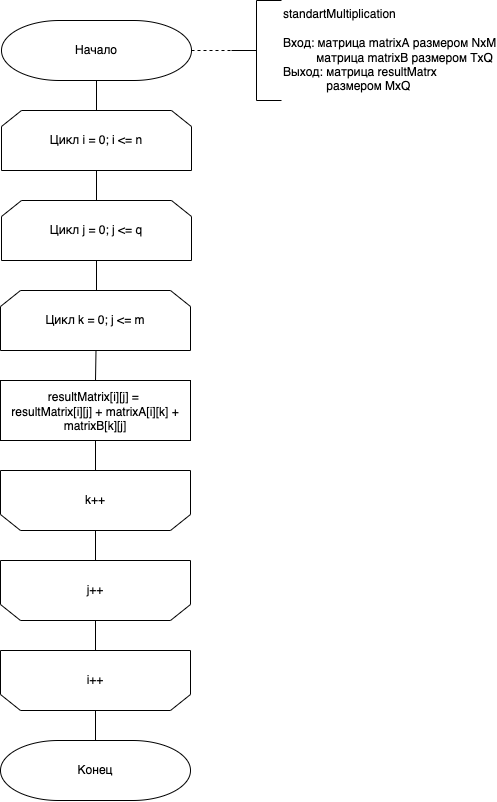
\includegraphics[width=0.9\linewidth]{img/Standard.png}
	\caption{Схема стандартного алгоритма умножения матриц}
	\label{fig:mpr}
\end{figure}

\newpage

\section{Парсинг http запросов}

Задача парсинга http запросов не относится к сути выполненной лабораторной работы и поэтому подробное описание алгоритма парсинга http запросов не приводится.



\section{Модель оценки эффективности серверного приложения}

Для оценки эффективности серверного приложения, разрабатываемого в рамках данной лабораторной работы, продложены следующие метрики: время обработки запросов в персентилях 50, 66, 75, 80, 90, 95, 98, 99, 100; количество запросов в секунду, при котором сервер может стабильно работать (rps).


